\documentclass[UTF8,12pt,AutoFakeBold]{ctexbook}

\usepackage{geometry}
\geometry{
	a4paper,
	total={170mm,257mm}, %设置页面尺寸
	left=25mm,
	right=25mm, %奇偶页边距一致
	top=20mm,
	bottom=20mm
}
\usepackage{multicol}
\usepackage{titlesec}
%改变章节标题样式
\titleformat{\chapter}[block]
{\normalfont\huge\bfseries}{Chapter \thechapter:}{1em}{}

%%%%%%%%%%%%数学%%%%%%%%%%%%%%%%
\usepackage{amsmath, amsfonts, amssymb, amsthm, mathrsfs}
\usepackage{witharrows}
\usepackage{enumitem}
\numberwithin{equation}{section}

%%%%%%%%%%%%表格%%%%%%%%%%%%
\usepackage{multirow, tabularx}

%%%%%%%%%%%%图片%%%%%%%%%%%%	
\usepackage{graphicx, float, subfigure}
\usepackage{subcaption}

%%%%%%%%%%%%算法%%%%%%%%%%%%
\usepackage{algorithm, algpseudocode}

%%%%%%%%%%%%盒子%%%%%%%%%%%%%
\usepackage{tikz, varwidth, mdframed, xcolor}
\usetikzlibrary{calc}
\usepackage[most]{tcolorbox}
\tcbuselibrary{xparse,hooks,skins,breakable,listings}
\input{box.tex}
\def\renewtheorem#1{%
	\expandafter\let\csname#1\endcsname\relax
	\expandafter\let\csname c@#1\endcsname\relax
	\gdef\renewtheorem@envname{#1}
	\renewtheorem@secpar
}
\def\renewtheorem@secpar{\@ifnextchar[{\renewtheorem@numberedlike}{\renewtheorem@nonumberedlike}}
\def\renewtheorem@numberedlike[#1]#2{\newtheorem{\renewtheorem@envname}[#1]{#2}}
\def\renewtheorem@nonumberedlike#1{
	\def\renewtheorem@caption{#1}
	\edef\renewtheorem@nowithin{\noexpand\newtheorem{\renewtheorem@envname}{\renewtheorem@caption}}
	\renewtheorem@thirdpar
}
\def\renewtheorem@thirdpar{\@ifnextchar[{\renewtheorem@within}{\renewtheorem@nowithin}}
\def\renewtheorem@within[#1]{\renewtheorem@nowithin[#1]}

\makeatother

%%%%%%%%%%%%%%%%%%%%
% New environments %
%%%%%%%%%%%%%%%%%%%%

\makeatother
\mdfsetup{skipabove=1em,skipbelow=0em}

\tcbuselibrary{skins}

% Color definitions

\definecolor{proofcolor}{RGB}{0,0,0}

% Dark orange and Dark Red rgb
\definecolor{theorembordercolor}{RGB}{151, 63, 5}
\definecolor{theorembackgroundcolor}{RGB}{248, 241, 234}

\definecolor{examplebordercolor}{RGB}{0, 110, 184}
\definecolor{examplebackgroundcolor}{RGB}{240, 244, 250}

\definecolor{definitionbordercolor}{RGB}{0, 150, 85}
\definecolor{definitionbackgroundcolor}{RGB}{239, 247, 243}

\definecolor{propertybordercolor}{RGB}{128, 0, 128}
\definecolor{propertybackgroundcolor}{RGB}{255, 240, 255}

\definecolor{formulabordercolor}{RGB}{0, 0, 0}
\definecolor{formulabackgroundcolor}{RGB}{230, 229, 245}

\newtheoremstyle{theorem}
{0pt}{0pt}{\normalfont}{0pt}
{}{\;}{0.25em}
{{\sffamily\bfseries\color{theorembordercolor}\thmname{#1}~\thmnumber{\textup{#2}}.}
	\thmnote{\normalfont\color{black}~(#3)}}

\newtheoremstyle{definition}
{0pt}{0pt}{\normalfont}{0pt}
{}{\;}{0.25em}
{{\sffamily\bfseries\color{definitionbordercolor}\thmname{#1}~\thmnumber{\textup{#2}}.}
	\thmnote{\normalfont\color{black}~(#3)}}

\newtheoremstyle{example}
{0pt}{0pt}{\normalfont}{0pt}
{}{\;}{0.25em}
{{\sffamily\bfseries\color{examplebordercolor}\thmname{#1}~\thmnumber{\textup{#2}}.}
	\thmnote{\normalfont\color{black}~(#3)}}

\newtheoremstyle{property}
{0pt}{0pt}{\normalfont}{0pt}
{}{\;}{0.25em}
{{\sffamily\bfseries\color{propertybordercolor}\thmname{#1}~\thmnumber{\textup{#2}}.}
	\thmnote{\normalfont\color{black}~(#3)}}

\newtheoremstyle{formula}
{0pt}{0pt}{\normalfont}{0pt}
{}{\;}{0.25em}
{{\sffamily\bfseries\color{formulabordercolor}\thmname{#1}~\thmnumber{\textup{#2}}.}
	\thmnote{\normalfont\color{black}~(#3)}}

%%%%%%%%%%%%%%%%%%%%%%%%
% Theorem Environments %
%%%%%%%%%%%%%%%%%%%%%%%%

\theoremstyle{theorem}

\newtheorem{theorem}{Theorem}[section]
\newtheorem{postulate}{Postulate}
\newtheorem{conjecture}{Conjecture}
\newtheorem{corollary}{Corollary}
\newtheorem{lemma}{Lemma}
\newtheorem{conclusion}{Conclusion}

\tcolorboxenvironment{theorem}{
	enhanced jigsaw, pad at break*=1mm, breakable,
	left=4mm, right=4mm, top=1mm, bottom=1mm,
	colback=theorembackgroundcolor, boxrule=0pt, frame hidden,
	borderline west={0.5mm}{0mm}{theorembordercolor}, arc=.5mm
}
\tcolorboxenvironment{postulate}{
	enhanced jigsaw, pad at break*=1mm, breakable,
	left=4mm, right=4mm, top=1mm, bottom=1mm,
	colback=theorembackgroundcolor, boxrule=0pt, frame hidden,
	borderline west={0.5mm}{0mm}{theorembordercolor}, arc=.5mm
}
\tcolorboxenvironment{conjecture}{
	enhanced jigsaw, pad at break*=1mm, breakable,
	left=4mm, right=4mm, top=1mm, bottom=1mm,
	colback=theorembackgroundcolor, boxrule=0pt, frame hidden,
	borderline west={0.5mm}{0mm}{theorembordercolor}, arc=.5mm
}
\tcolorboxenvironment{corollary}{
	enhanced jigsaw, pad at break*=1mm, breakable,
	left=4mm, right=4mm, top=1mm, bottom=1mm,
	colback=theorembackgroundcolor, boxrule=0pt, frame hidden,
	borderline west={0.5mm}{0mm}{theorembordercolor}, arc=.5mm
}
\tcolorboxenvironment{lemma}{
	enhanced jigsaw, pad at break*=1mm, breakable,
	left=4mm, right=4mm, top=1mm, bottom=1mm,
	colback=theorembackgroundcolor, boxrule=0pt, frame hidden,
	borderline west={0.5mm}{0mm}{theorembordercolor}, arc=.5mm
}
\tcolorboxenvironment{conclusion}{
	enhanced jigsaw, pad at break*=1mm, breakable,
	left=4mm, right=4mm, top=1mm, bottom=1mm,
	colback=theorembackgroundcolor, boxrule=0pt, frame hidden,
	borderline west={0.5mm}{0mm}{theorembordercolor}, arc=.5mm
}

%%%%%%%%%%%%%%%%%%%%%%%%%%%
% Definition Environments %
%%%%%%%%%%%%%%%%%%%%%%%%%%%

\theoremstyle{definition}
\newtheorem{definition}{Definition}[section]
\newtheorem{review}{Review}

\tcolorboxenvironment{definition}{
	enhanced jigsaw, pad at break*=1mm, breakable,
	left=4mm, right=4mm, top=1mm, bottom=1mm,
	colback=definitionbackgroundcolor, boxrule=0pt, frame hidden,
	borderline west={0.5mm}{0mm}{definitionbordercolor}, arc=.5mm
}
\tcolorboxenvironment{review}{
	enhanced jigsaw, pad at break*=1mm, breakable,
	left=4mm, right=4mm, top=1mm, bottom=1mm,
	colback=definitionbackgroundcolor, boxrule=0pt, frame hidden,
	borderline west={0.5mm}{0mm}{definitionbordercolor}, arc=.5mm
}


%%%%%%%%%%%%%%%%%%%%%%%%
% Example Environments %
%%%%%%%%%%%%%%%%%%%%%%%%

\theoremstyle{example}
\newtheorem{example}{Example}[section]
\newtheorem{remark}{Remark}
\newtheorem{note}{Note}

\tcolorboxenvironment{example}{
	enhanced jigsaw, pad at break*=1mm, breakable,
	left=4mm, right=4mm, top=1mm, bottom=1mm,
	colback=examplebackgroundcolor, boxrule=0pt, frame hidden,
	borderline west={0.5mm}{0mm}{examplebordercolor}, arc=.5mm
}
\tcolorboxenvironment{remark}{
	enhanced jigsaw, pad at break*=1mm, breakable,
	left=4mm, right=4mm, top=1mm, bottom=1mm,
	colback=white, boxrule=0pt, frame hidden,
	borderline west={0.5mm}{0mm}{examplebordercolor}, arc=.5mm
}
\tcolorboxenvironment{note}{
	enhanced jigsaw, pad at break*=1mm, breakable,
	left=4mm, right=4mm, top=1mm, bottom=1mm,
	colback=white, boxrule=0pt, frame hidden,
	borderline west={0.5mm}{0mm}{examplebordercolor}, arc=.5mm
}


%%%%%%%%%%%%%%%%%%%%%%%%%
% Property Environments %
%%%%%%%%%%%%%%%%%%%%%%%%%

\theoremstyle{property}
\newtheorem{property}{Property}[section]
\newtheorem{proposition}{Proposition}[section]

\tcolorboxenvironment{property}{
	enhanced jigsaw, pad at break*=1mm, breakable,
	left=4mm, right=4mm, top=1mm, bottom=1mm,
	colback=propertybackgroundcolor, boxrule=0pt, frame hidden,
	borderline west={0.5mm}{0mm}{propertybordercolor}, arc=.5mm
}
\tcolorboxenvironment{proposition}{
	enhanced jigsaw, pad at break*=1mm, breakable,
	left=4mm, right=4mm, top=1mm, bottom=1mm,
	colback=propertybackgroundcolor, boxrule=0pt, frame hidden,
	borderline west={0.5mm}{0mm}{propertybordercolor}, arc=.5mm
}

%%%%%%%%%%%%
% Formula %
%%%%%%%%%%%%

\theoremstyle{formula}
\newtheorem{formula}{Formula}[section]

\tcolorboxenvironment{formula}{
	enhanced jigsaw, pad at break*=1mm, breakable,
	left=4mm, right=4mm, top=1mm, bottom=1mm,
	colback=formulabackgroundcolor, boxrule=0pt, frame hidden,
	borderline west={0.5mm}{0mm}{formulabordercolor}, arc=.5mm
}

%%%%%%%%%
% Proof %
%%%%%%%%%

% These patches must be placed after \tcolorboxenvironment !
\AddToHook{env/theorem/after}{\colorlet{proofcolor}{theorembordercolor}}
\AddToHook{env/postulate/after}{\colorlet{proofcolor}{theorembordercolor}}
\AddToHook{env/conjecture/after}{\colorlet{proofcolor}{theorembordercolor}}
\AddToHook{env/corollary/after}{\colorlet{proofcolor}{theorembordercolor}}
\AddToHook{env/lemma/after}{\colorlet{proofcolor}{theorembordercolor}}
\AddToHook{env/conclusion/after}{\colorlet{proofcolor}{theorembordercolor}}

\AddToHook{env/definition/after}{\colorlet{proofcolor}{definitionbordercolor}}
\AddToHook{env/review/after}{\colorlet{proofcolor}{definitionbordercolor}}

\AddToHook{env/example/after}{\colorlet{proofcolor}{examplebordercolor}}
\AddToHook{env/remark/after}{\colorlet{proofcolor}{examplebordercolor}}
\AddToHook{env/note/after}{\colorlet{proofcolor}{examplebordercolor}}

\AddToHook{env/property/after}{\colorlet{proofcolor}{propertybordercolor}}
\AddToHook{env/proposition/after}{\colorlet{proofcolor}{propertybordercolor}}

\AddToHook{env/formula/after}{\colorlet{proofcolor}{formulabordercolor}}

\renewcommand{\qedsymbol}{$\square$}
\let\qedsymbolMyOriginal\qedsymbol
\renewcommand{\qedsymbol}{
	\color{proofcolor}\qedsymbolMyOriginal
}

\newtheoremstyle{proof}
{0pt}{0pt}{\normalfont}{0pt}
{}{\;}{0.25em}
{{\sffamily\bfseries\color{proofcolor}\thmname{#1}.}
	\thmnote{\normalfont\color{black}~(\textit{#3})}}

\theoremstyle{proof}
%\renewtheorem{proof}{Proof}

\tcolorboxenvironment{proof}{
	enhanced jigsaw, pad at break*=1mm, breakable,
	left=4mm, right=4mm, top=1mm, bottom=1mm,
	colback=white, boxrule=0pt, frame hidden,
	%borderline west={0.5mm}{0mm}{proofcolor}, arc=.5mm
}

\newenvironment{info}{\begin{tcolorbox}[
		arc=0mm,
		colback=white,
		colframe=gray,
		title=Info,
		fonttitle=\sffamily,
		breakable
		]}{\end{tcolorbox}}
\newenvironment{terminology}{\begin{tcolorbox}[
		arc=0mm,
		colback=white,
		colframe=green!60!black,
		title=Terminology,
		fonttitle=\sffamily,
		breakable
		]}{\end{tcolorbox}}
\newenvironment{warning}{\begin{tcolorbox}[
		arc=0mm,
		colback=white,
		colframe=red,
		title=Warning,
		fonttitle=\sffamily,
		breakable
		]}{\end{tcolorbox}}
\newenvironment{caution}{\begin{tcolorbox}[
		arc=0mm,
		colback=white,
		colframe=yellow,
		title=Caution,
		fonttitle=\sffamily,
		breakable
		]}{\end{tcolorbox}}

\definecolor{citecolor}{RGB}{60,120,216}
\definecolor{urlcolor}{RGB}{60,120,216}
\definecolor{linkcolor}{RGB}{60,120,216}

%%%%%%%%%%%%超链接%%%%%%%%%%%%%
\usepackage{hyperref}
\hypersetup{
	colorlinks=true,
	linkcolor=linkcolor,
	urlcolor=urlcolor,
	%allcolors=blue,
	citecolor=cyan,
	pdftitle={Real Analysis},
	%linkcolor=blue,
	filecolor=magenta,      
	%urlcolor=cyan,
}

%%%%%%%%%%%%参考文献%%%%%%%%%%%%%
\usepackage[round]{natbib}
\bibliographystyle{unsrtnat}

%%%%%%%%%%%%其他%%%%%%%%%%%%%
\usepackage[english]{babel}
\usepackage{caption, marginnote, lipsum, ifthen}

\definecolor{mynotecolor}{rgb}{0.6, 0.4, 0.2}
\newcommand{\mymarginnote}[1]{
	\ifthenelse{\isodd{\value{page}}}
	{\normalmarginpar\marginnote{\textcolor{mynotecolor}{#1}}}
	{\reversemarginpar\marginnote{\textcolor{mynotecolor}{#1}}}
}

\title{Notes of Real Analysis}
\author{Renhe W.}
\date{}

%文章开始部分
\begin{document}
	\maketitle
	\tableofcontents
	
	\newpage
	\kaishu
	%引言
	\section{Introduction}
	This note is to provide an easy understanding of Real Analysis, and to continue to understand and work on more specific areas. And the content are almost come from \href{https://www.bilibili.com/video/BV1FT411C7wM/?spm_id_from=333.337.search-card.all.click&vd_source=ba9c3e9308deddcceb8190c43ed27dfd}{bilibili}
	
	
	\chapter{Abstract Measures}
	\section{Building Block}
	
	\subsection{Rectangles}
	\begin{definition}[closed rectangle]
		A \textbf{closed rectangle} $R$ in $\mathbb{R}^d$ is defined as the Cartesian product of closed intervals. Specifically, $R$ can be written as:
		$$
		R=\left[a_1, b_1\right] \times\left[a_2, b_2\right] \times \cdots \times\left[a_d, b_d\right],
		$$
		where $\left[a_i, b_i\right]$ are closed intervals on the real line, and $a_i \leq b_i$ for all $i$ from 1 to $d$.
		
		In other words,
		$$
		R = \{(X_1,X_2,\dots,X_d)\in\mathbb{R}^d:a_j\leq b_j, j = 1,\dots,d\},
		$$
		The {\color{blue}volume} of $R$ is
		$$
			\left | R \right | = \left(b_1-a_1\right) \times \left(b_2-a_2\right) \times \cdots \times\left(b_d-a_d\right),
		$$
		An \textbf{open rectangle} is the product of open intervals, and the interior of the rectangle $R$ is
		$$
			\left(a_1, b_1\right) \times\left(a_2, b_2\right) \times \cdots \times\left(a_d, b_d\right).
		$$
	\end{definition}
	
	\begin{example}[Closed Rectangles]There are some examples of \textbf{closed rectangle}:
		\begin{enumerate}
			\item  In $\mathbb{R}^2$ (the plane), a building block might be a rectangle defined by $R=[1,3] \times[2,4]$. This rectangle includes all points $(x, y)$ where $1 \leq x \leq 3$ and $2 \leq y \leq 4$.
			\begin{figure}[H] 
				\centering  
			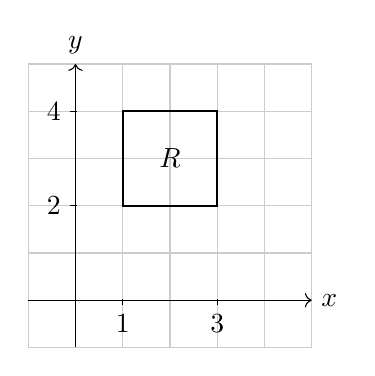
\begin{tikzpicture}[scale=0.6]
				% Draw the axes
				\draw[thin,gray!40] (-1,-1) grid (5,5);
				\draw[->] (-1,0)--(5,0) node[right]{$x$};
				\draw[->] (0,-1)--(0,5) node[above]{$y$};
				
				% Draw the rectangle with points and labels
				\draw[thick] (1,2) rectangle (3,4);
				\foreach \x/\xtext in {1, 3}
				\draw (\x,1pt) -- (\x,-3pt) node[anchor=north] {$\x$};
				\foreach \y/\ytext in {2, 4}
				\draw (1pt,\y) -- (-3pt,\y) node[anchor=east] {$\y$};
				
				% Label the rectangle
				\node at (2,3) {$R$};
			\end{tikzpicture}
			 \caption{The rectangle $R = [1, 3] \times [2, 4]$ in $\mathbb{R}^2$}
			\end{figure}
			\item  In $\mathbb{R}^3$ (three-dimensional space), a typical building block could be a rectangular prism (or box) defined by $R=[0,1] \times[0,1] \times[0,1]$. This includes all points $(x, y, z)$ where $0 \leq x \leq 1,0 \leq y \leq 1$, and $0 \leq z \leq 1$.
		\end{enumerate}
	\end{example}
	
	\begin{definition}[Almost Disjoint]
		A union of rectangles is said to be {\color{blue}almost disjoint} if the interiors of them are disjoint.
	\end{definition}
	
	\begin{figure}[H]
		\centering
		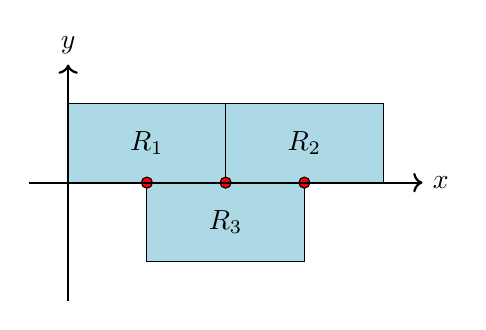
\begin{tikzpicture}
			% Define colors for visibility
			\definecolor{lightblue}{RGB}{173,216,230}
			
			% Draw the first rectangle
			\filldraw[fill=lightblue, draw=black] (0,0) rectangle (2,1);
			\node at (1, 0.5) {$R_1$};
			
			% Draw the second rectangle
			\filldraw[fill=lightblue, draw=black] (2,0) rectangle (4,1);
			\node at (3, 0.5) {$R_2$};
			
			% Draw the third rectangle
			\filldraw[fill=lightblue, draw=black] (1,-1) rectangle (3,0);
			\node at (2, -0.5) {$R_3$};
			
			% Label the touching points
			\draw[fill=red] (2,0) circle (2pt);
			\draw[fill=red] (1,0) circle (2pt);
			\draw[fill=red] (3,0) circle (2pt);
			
			% Draw axes (optional, for reference)
			\draw[thick,->] (-0.5,0) -- (4.5,0) node[right] {$x$};
			\draw[thick,->] (0,-1.5) -- (0,1.5) node[above] {$y$};
		\end{tikzpicture}
	\end{figure}
	The rectangle $R_1$ and $R_2$ share a common boundary along the line $x=2$ but do not overlap. $R_3$ is positioned such that it touches the bottom edges of $R_1$ and $R_2$ at points along the line $y=0$. The points where the rectangles touch are highlighted with red dots to emphasize the boundary interactions but no interior overlap.
	\begin{lemma}
		If a rectangles is the almost disjoint union of finitely many rectangles: $R=\bigcup_{N}^{k=1} R_k $, then $\left | R \right |=\sum_{k=1}^{N}\left | R_k \right |$.
	\end{lemma}
	这个引理描述了一种特殊情况,其中一个矩形 \( R \) 是有限个几乎不相交的矩形的并集,即 \( R=\bigcup_{k=1}^N R_k \),并且这些矩形的内部不相交. 在这种情况下,\( R \) 的体积等于所有这些子矩形体积的总和.
	\begin{proof}
		定义每个 \( R_k \) 为闭矩形 \([a_{k1}, b_{k1}] \times [a_{k2}, b_{k2}] \times \cdots \times [a_{kd}, b_{kd}]\), 对于任何 \( i \neq j \),\( \text{int}(R_i) \cap \text{int}(R_j) = \emptyset \). \marginnote{\tiny Almost Disjoint}其中每个 \( R_k \) 的体积计算为 \( |R_k| = \prod_{j=1}^d (b_{kj} - a_{kj}) \).
		
		设 \( R = [a_1, b_1] \times [a_2, b_2] \times \cdots \times [a_d, b_d] \),其中 \( a_j = \min_k a_{kj} \),\( b_j = \max_k b_{kj} \)\marginnote{\tiny 最小包含矩形 \( R \)}.
		
		由于 \( \text{int}(R_i) \cap \text{int}(R_j) = \emptyset \),可以断定每个 \( R_k \) 的体积贡献是独立的,即它们的体积之和给出了 \( R \) 中被覆盖的全部体积.
		
		\( R_k \) 的边界可能与其他 \( R_k \) 的边界重合,但由于边界的测度在整体测度中不起主导作用(在高维中测度为零),因此不影响总体积计算.
		
		因此,可以通过各 \( R_k \) 的体积独立累加,无需减去重叠部分,从而得到 \( R \) 的总体积,即 \( |R| = \sum_{k=1}^N |R_k| \).
	\end{proof}
	
	\begin{lemma}
		If $R, R_1,\dots, R_N$ are rectangles, and $R \subset \bigcup_{N}^{k=1}R_k$, then
		$$
		\left | R \right | \le  \sum_{k=1}^{N}\left | R_k \right |.
		$$
		
	\end{lemma}
	
	
	\begin{figure}[H]
		\centering
		\tikzset{every picture/.style={line width=0.75pt}} %set default line width to 0.75pt        
		
		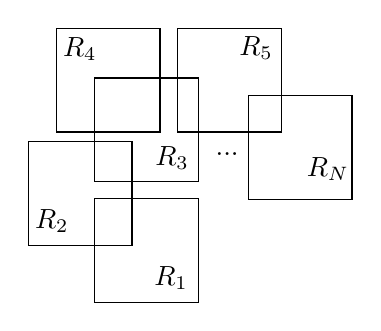
\begin{tikzpicture}[x=0.75pt,y=0.75pt,yscale=-1,xscale=1]
			%uncomment if require: \path (0,300); %set diagram left start at 0, and has height of 300
			
			%Shape: Square [id:dp8186847949108236] 
			\draw   (170,100.5) -- (220,100.5) -- (220,150.5) -- (170,150.5) -- cycle ;
			%Shape: Square [id:dp5111877257315434] 
			\draw   (202,128) -- (252,128) -- (252,178) -- (202,178) -- cycle ;
			%Shape: Square [id:dp48467482655549166] 
			\draw   (202,70) -- (252,70) -- (252,120) -- (202,120) -- cycle ;
			%Shape: Square [id:dp14981018840115534] 
			\draw   (183.5,46) -- (233.5,46) -- (233.5,96) -- (183.5,96) -- cycle ;
			%Shape: Square [id:dp4244294715215631] 
			\draw   (242,46) -- (292,46) -- (292,96) -- (242,96) -- cycle ;
			%Shape: Square [id:dp6675999695494248] 
			\draw   (276,78.5) -- (326,78.5) -- (326,128.5) -- (276,128.5) -- cycle ;
			
			% Text Node
			\draw (229.5,159.4) node [anchor=north west][inner sep=0.75pt]    {$R_{1}$};
			% Text Node
			\draw (172,131.9) node [anchor=north west][inner sep=0.75pt]    {$R_{2}$};
			% Text Node
			\draw (230,101.9) node [anchor=north west][inner sep=0.75pt]    {$R_{3}$};
			% Text Node
			\draw (259,104.5) node [anchor=north west][inner sep=0.75pt]   [align=left] {...};
			% Text Node
			\draw (185.5,49.4) node [anchor=north west][inner sep=0.75pt]    {$R_{4}$};
			% Text Node
			\draw (270.5,48.9) node [anchor=north west][inner sep=0.75pt]    {$R_{5}$};
			% Text Node
			\draw (303,106.9) node [anchor=north west][inner sep=0.75pt]    {$R_{N}$};
					
		\end{tikzpicture}
	\end{figure}
	
	The main idea consists of taking the grid formed by extending all sides of the rectangles $R, R_1, \ldots, R_N$, and noting that the sets corresponding to the $J_k$ (in the above proof) need not be disjoint any more.


	\subsection{Open Sets}
	
	\begin{theorem}[Open Sets]
		Every \textbf{open set} $O$ of $\mathbb{R}$ can be written uniquely as a countable union of disjoint open intervals.
	\end{theorem}
	
	\begin{proof}
		Let $O \subseteq \mathbb{R}$ be open and let $x \in O$. Then Either $x$ is rational or $x$ is irrational.
		Suppose $x$ is rational, then define
		
		$$
		I_x=\bigcup_{\substack{\text { an open interval } \\ x \in I \subseteq O}} I
		$$
		
		\textbf{Claim:} $I_x$ is interval, $I_x$ is open and $I_x \subseteq O$.
		
		\textbf{Definition:} An interval is a subset $I \subseteq \mathbb{R}$ such that, for all $a<c<b$ in $\mathbb{R}$, if $a, b \in I$ then $c \in I$.
		
		Now, consider any $a<c<b$ such that $a, b \in I_x$. We want to show that $c \in I_x$.
		Denote $I_a$ to be an interval such that $x \in I_a$ and $a \in I_a$. In other words $I_a$ is one of the intervals from the union $I_x$ that contains $a$. In the same way, let $I_b$ be the interval such that $x \in I_b$ and $b \in I_b$.
		\begin{enumerate}
			\item $c=x$. If $c=x$ then by construction of $I_x, c \in I_x$.
			\item $c<x$ : If $c<x$ then we have that either $a<c<x<b$ or $a<c<b<x$. Since $x \in I$ for every open interval $I$ of the union $I_x$ (by construction of $I_x$ ), we have that $x \in I_a$ and $x \in I_b$. Since $x \in I_a$ then because $I_a$ is an interval $c \in I_a$ and hence $c \in I_x$. And since $x \in I_b$ then because $I_b$ is an interval $c \in I_b$ and hence $c \in I_x$. Thus, we concluded that $c \in I_x$. 
			\item  $c>x$ : If $c>x$ then we have that either $a<x<c<b$ or $x<a<c<b$. Since $x \in I$ for every open interval $I$ of the union $I_x$ (by construction of $I_x$ ), we have that $x \in I_a$ and $x \in I_b$. Since $x \in I_b$ then because $I_b$ is an interval $c \in I_b$ and hence $c \in I_x$. As for the second case, note that since $x \in I_b$ we have that $a \in I_b$. But then, because $I_b$ is an interval we have that $c \in I_b$ and hence $c \in I_x$. Hence we concluded that $c \in I_x$.
		\end{enumerate}
	
		This Proves that
		
		\begin{itemize}
			\item $I_x$ is an interval.
			\item $I_x$ is open because it is union of open sets.
			\item $I_x \subseteq O$ by construction.
		\end{itemize}
		
		Suppose $x$ is irrational, then by openness of $O$ there is $\varepsilon>0$ such that $(x-\varepsilon, x+\varepsilon) \subseteq U$, and by the property of real numbers that for any irrational number there exists a sequence of rational unmbers that converges to that irrational number, there exists rational $y \in(x-\varepsilon, x+\varepsilon)$. Then by construction $(x-\varepsilon, x+\varepsilon) \subseteq I_y$. Hence $x \in I_y$. So any $x \in O$ is in $I_q$ for some $q \in O \cap \mathbb{Q}$, and so
		
		$$
		O \subseteq \bigcup_{q \in O \cap \mathbb{Q}} I_q
		$$
		
		
		But $I_q \subseteq O$ for each $q \in O \cap \mathbb{Q}$; thus
		
		$$
		O=\bigcup_{q \in O \cap \mathbb{Q}} I_q
		$$
		
		which is a countable union of open intervals.
		
		
		Now let's show that intervals $\left\{I_q\right\} \quad q \in O \cap \mathbb{Q}$ are disjoint. Suppose there is $i, j, \in O \cap \mathbb{Q}$ such that $I_i \cap I_j \neq \emptyset$ then $I_i \subseteq I_q$ and $I_j \subseteq I_q$ for some $q \in O \cap \mathbb{Q}$
		
		Hence we constructed disjoint intervals $\left\{I_q\right\} \quad q \in O \cap \mathbb{Q}$ that are enumerated by rational numbers in $O$ and whose union is $O$. Since any subset of rational numbers is countable, $\left\{I_q\right\} q \in O \cap \mathbb{Q}$ is countable as well. This finishes the proof.
		
		
	\end{proof}
	
	\begin{theorem}
		Every \textbf{open set} $O$ of $\mathbb{R}^d$ ($d\ge 1$) can be written as a countable union of almost disjoint {\color{blue}closed cubes}.
	\end{theorem}
	
	\begin{proof}
		 We must construct a countable collection $\mathcal{Q}$ of closed cubes whose interiors are disjoint, and so that $O=\bigcup_{Q \in \mathcal{Q}} Q$.
		
		As a first step, consider the grid in $\mathbb{R}^d$ formed by taking all closed cubes of side length 1 whose vertices have integer coordinates. In other words, we consider the natural grid of lines parallel to the axes, that is, the grid generated by the lattice $\mathbb{Z}^d$. We shall also use the grids formed by cubes of side length $2^{-N}$ obtained by successively bisecting the original grid.
		
		We either accept or reject cubes in the initial grid as part of $\mathcal{Q}$ according to the following rule: if $Q$ is entirely contained in $O$ then we accept $Q$; if $Q$ intersects both $\O$ and $O^c$ then we tentatively accept it; and if $Q$ is entirely contained in $O^c$ then we reject it.
		
		As a second step, we bisect the tentatively accepted cubes into $2^d$ cubes with side length $1 / 2$. We then repeat our procedure, by accepting the smaller cubes if they are completely contained in $O$, tentatively accepting them if they intersect both $O$ and $O^c$, and rejecting them if they are contained in $O^c$. The following Figure illustrates these steps for an open set in $\mathbb{R}^2$.
		
		\begin{multicols}{2}
			\begin{figure}[H]
				\centering
				\tikzset{every picture/.style={line width=0.75pt}} %set default line width to 0.75pt        
				
				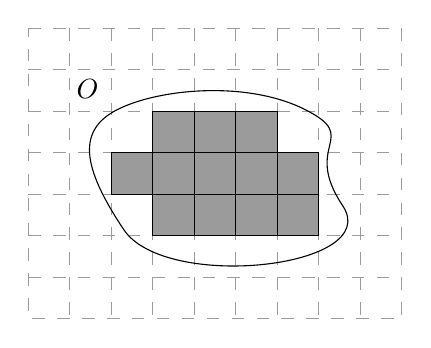
\begin{tikzpicture}[x=0.75pt,y=0.75pt,yscale=-1,xscale=1]
					%uncomment if require: \path (0,300); %set diagram left start at 0, and has height of 300
					
					%Shape: Grid [id:dp3822292598133501] 
					\draw  [draw opacity=0][dash pattern={on 4.5pt off 4.5pt}] (107.83,44.42) -- (287.83,44.42) -- (287.83,184.42) -- (107.83,184.42) -- cycle ; \draw  [color={rgb, 255:red, 155; green, 155; blue, 155 }  ,draw opacity=1 ][dash pattern={on 4.5pt off 4.5pt}] (127.83,44.42) -- (127.83,184.42)(147.83,44.42) -- (147.83,184.42)(167.83,44.42) -- (167.83,184.42)(187.83,44.42) -- (187.83,184.42)(207.83,44.42) -- (207.83,184.42)(227.83,44.42) -- (227.83,184.42)(247.83,44.42) -- (247.83,184.42)(267.83,44.42) -- (267.83,184.42) ; \draw  [color={rgb, 255:red, 155; green, 155; blue, 155 }  ,draw opacity=1 ][dash pattern={on 4.5pt off 4.5pt}] (107.83,64.42) -- (287.83,64.42)(107.83,84.42) -- (287.83,84.42)(107.83,104.42) -- (287.83,104.42)(107.83,124.42) -- (287.83,124.42)(107.83,144.42) -- (287.83,144.42)(107.83,164.42) -- (287.83,164.42) ; \draw  [color={rgb, 255:red, 155; green, 155; blue, 155 }  ,draw opacity=1 ][dash pattern={on 4.5pt off 4.5pt}] (107.83,44.42) -- (287.83,44.42) -- (287.83,184.42) -- (107.83,184.42) -- cycle ;
					%Shape: Polygon Curved [id:ds06871142337325908] 
					\draw   (151,83.5) .. controls (171,73.5) and (213.17,69.58) .. (241,83.5) .. controls (268.83,97.42) and (239.33,99.92) .. (259.33,129.92) .. controls (279.33,159.92) and (173.83,171.42) .. (153.83,141.42) .. controls (133.83,111.42) and (131,93.5) .. (151,83.5) -- cycle ;
					%Shape: Square [id:dp7122260258712552] 
					\draw  [fill={rgb, 255:red, 155; green, 155; blue, 155 }  ,fill opacity=1 ] (167.83,84.42) -- (187.83,84.42) -- (187.83,104.42) -- (167.83,104.42) -- cycle ;
					%Shape: Square [id:dp261607807338875] 
					\draw  [fill={rgb, 255:red, 155; green, 155; blue, 155 }  ,fill opacity=1 ] (187.83,104.42) -- (207.83,104.42) -- (207.83,124.42) -- (187.83,124.42) -- cycle ;
					%Shape: Square [id:dp8667533091763637] 
					\draw  [fill={rgb, 255:red, 155; green, 155; blue, 155 }  ,fill opacity=1 ] (187.83,124.42) -- (207.83,124.42) -- (207.83,144.42) -- (187.83,144.42) -- cycle ;
					%Shape: Square [id:dp24613434128777922] 
					\draw  [fill={rgb, 255:red, 155; green, 155; blue, 155 }  ,fill opacity=1 ] (207.83,124.42) -- (227.83,124.42) -- (227.83,144.42) -- (207.83,144.42) -- cycle ;
					%Shape: Square [id:dp40897704856741113] 
					\draw  [fill={rgb, 255:red, 155; green, 155; blue, 155 }  ,fill opacity=1 ] (207.83,104.42) -- (227.83,104.42) -- (227.83,124.42) -- (207.83,124.42) -- cycle ;
					%Shape: Square [id:dp05460497539097764] 
					\draw  [fill={rgb, 255:red, 155; green, 155; blue, 155 }  ,fill opacity=1 ] (227.83,124.42) -- (247.83,124.42) -- (247.83,144.42) -- (227.83,144.42) -- cycle ;
					%Shape: Square [id:dp13132167195455224] 
					\draw  [fill={rgb, 255:red, 155; green, 155; blue, 155 }  ,fill opacity=1 ] (227.83,104.42) -- (247.83,104.42) -- (247.83,124.42) -- (227.83,124.42) -- cycle ;
					%Shape: Square [id:dp7248205668607259] 
					\draw  [fill={rgb, 255:red, 155; green, 155; blue, 155 }  ,fill opacity=1 ] (187.83,84.42) -- (207.83,84.42) -- (207.83,104.42) -- (187.83,104.42) -- cycle ;
					%Shape: Square [id:dp22082507490517567] 
					\draw  [fill={rgb, 255:red, 155; green, 155; blue, 155 }  ,fill opacity=1 ] (207.83,84.42) -- (227.83,84.42) -- (227.83,104.42) -- (207.83,104.42) -- cycle ;
					%Shape: Square [id:dp24418775213301447] 
					\draw  [fill={rgb, 255:red, 155; green, 155; blue, 155 }  ,fill opacity=1 ] (167.83,104.42) -- (187.83,104.42) -- (187.83,124.42) -- (167.83,124.42) -- cycle ;
					%Shape: Square [id:dp5822986921822859] 
					\draw  [fill={rgb, 255:red, 155; green, 155; blue, 155 }  ,fill opacity=1 ] (147.83,104.42) -- (167.83,104.42) -- (167.83,124.42) -- (147.83,124.42) -- cycle ;
					%Shape: Square [id:dp1808475363152242] 
					\draw  [fill={rgb, 255:red, 155; green, 155; blue, 155 }  ,fill opacity=1 ] (167.83,124.42) -- (187.83,124.42) -- (187.83,144.42) -- (167.83,144.42) -- cycle ;
					
					% Text Node
					\draw (129.83,67.82) node [anchor=north west][inner sep=0.75pt]    {$O$};		
				\end{tikzpicture}
				\caption{Step 1}
				%\label{fig:step1}
			\end{figure}
			
			\begin{figure}[H]
			\centering
			\tikzset{every picture/.style={line width=0.75pt}} %set default line width to 0.75pt        
			
			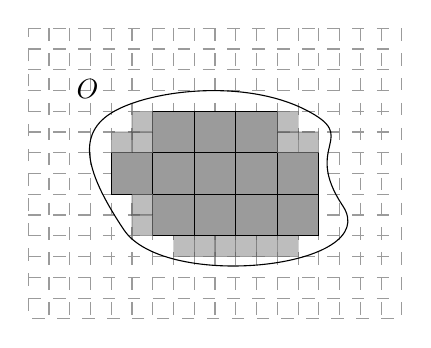
\begin{tikzpicture}[x=0.75pt,y=0.75pt,yscale=-1,xscale=1]
				%uncomment if require: \path (0,300); %set diagram left start at 0, and has height of 300
				
				%Shape: Grid [id:dp4257450376627836] 
				\draw  [draw opacity=0][dash pattern={on 4.5pt off 4.5pt}] (333.33,41.92) -- (513.33,41.92) -- (513.33,181.92) -- (333.33,181.92) -- cycle ; \draw  [color={rgb, 255:red, 155; green, 155; blue, 155 }  ,draw opacity=1 ][dash pattern={on 4.5pt off 4.5pt}] (343.33,41.92) -- (343.33,181.92)(353.33,41.92) -- (353.33,181.92)(363.33,41.92) -- (363.33,181.92)(373.33,41.92) -- (373.33,181.92)(383.33,41.92) -- (383.33,181.92)(393.33,41.92) -- (393.33,181.92)(403.33,41.92) -- (403.33,181.92)(413.33,41.92) -- (413.33,181.92)(423.33,41.92) -- (423.33,181.92)(433.33,41.92) -- (433.33,181.92)(443.33,41.92) -- (443.33,181.92)(453.33,41.92) -- (453.33,181.92)(463.33,41.92) -- (463.33,181.92)(473.33,41.92) -- (473.33,181.92)(483.33,41.92) -- (483.33,181.92)(493.33,41.92) -- (493.33,181.92)(503.33,41.92) -- (503.33,181.92) ; \draw  [color={rgb, 255:red, 155; green, 155; blue, 155 }  ,draw opacity=1 ][dash pattern={on 4.5pt off 4.5pt}] (333.33,51.92) -- (513.33,51.92)(333.33,61.92) -- (513.33,61.92)(333.33,71.92) -- (513.33,71.92)(333.33,81.92) -- (513.33,81.92)(333.33,91.92) -- (513.33,91.92)(333.33,101.92) -- (513.33,101.92)(333.33,111.92) -- (513.33,111.92)(333.33,121.92) -- (513.33,121.92)(333.33,131.92) -- (513.33,131.92)(333.33,141.92) -- (513.33,141.92)(333.33,151.92) -- (513.33,151.92)(333.33,161.92) -- (513.33,161.92)(333.33,171.92) -- (513.33,171.92) ; \draw  [color={rgb, 255:red, 155; green, 155; blue, 155 }  ,draw opacity=1 ][dash pattern={on 4.5pt off 4.5pt}] (333.33,41.92) -- (513.33,41.92) -- (513.33,181.92) -- (333.33,181.92) -- cycle ;
				%Shape: Polygon Curved [id:ds48730777214041554] 
				\draw   (376.5,81) .. controls (396.5,71) and (438.67,67.08) .. (466.5,81) .. controls (494.33,94.92) and (464.83,97.42) .. (484.83,127.42) .. controls (504.83,157.42) and (399.33,168.92) .. (379.33,138.92) .. controls (359.33,108.92) and (356.5,91) .. (376.5,81) -- cycle ;
				%Shape: Square [id:dp44246129760130826] 
				\draw  [fill={rgb, 255:red, 155; green, 155; blue, 155 }  ,fill opacity=1 ] (393.33,81.92) -- (413.33,81.92) -- (413.33,101.92) -- (393.33,101.92) -- cycle ;
				%Shape: Square [id:dp8412970131506399] 
				\draw  [fill={rgb, 255:red, 155; green, 155; blue, 155 }  ,fill opacity=1 ] (413.33,101.92) -- (433.33,101.92) -- (433.33,121.92) -- (413.33,121.92) -- cycle ;
				%Shape: Square [id:dp13943749929677018] 
				\draw  [fill={rgb, 255:red, 155; green, 155; blue, 155 }  ,fill opacity=1 ] (413.33,121.92) -- (433.33,121.92) -- (433.33,141.92) -- (413.33,141.92) -- cycle ;
				%Shape: Square [id:dp7700741522985384] 
				\draw  [fill={rgb, 255:red, 155; green, 155; blue, 155 }  ,fill opacity=1 ] (433.33,121.92) -- (453.33,121.92) -- (453.33,141.92) -- (433.33,141.92) -- cycle ;
				%Shape: Square [id:dp4682677469421548] 
				\draw  [fill={rgb, 255:red, 155; green, 155; blue, 155 }  ,fill opacity=1 ] (433.33,101.92) -- (453.33,101.92) -- (453.33,121.92) -- (433.33,121.92) -- cycle ;
				%Shape: Square [id:dp6103817441077295] 
				\draw  [fill={rgb, 255:red, 155; green, 155; blue, 155 }  ,fill opacity=1 ] (453.33,121.92) -- (473.33,121.92) -- (473.33,141.92) -- (453.33,141.92) -- cycle ;
				%Shape: Square [id:dp6396795848338577] 
				\draw  [fill={rgb, 255:red, 155; green, 155; blue, 155 }  ,fill opacity=1 ] (453.33,101.92) -- (473.33,101.92) -- (473.33,121.92) -- (453.33,121.92) -- cycle ;
				%Shape: Square [id:dp6256497649764732] 
				\draw  [fill={rgb, 255:red, 155; green, 155; blue, 155 }  ,fill opacity=1 ] (413.33,81.92) -- (433.33,81.92) -- (433.33,101.92) -- (413.33,101.92) -- cycle ;
				%Shape: Square [id:dp07142699585816326] 
				\draw  [fill={rgb, 255:red, 155; green, 155; blue, 155 }  ,fill opacity=1 ] (433.33,81.92) -- (453.33,81.92) -- (453.33,101.92) -- (433.33,101.92) -- cycle ;
				%Shape: Square [id:dp05255529242189505] 
				\draw  [fill={rgb, 255:red, 155; green, 155; blue, 155 }  ,fill opacity=1 ] (393.33,101.92) -- (413.33,101.92) -- (413.33,121.92) -- (393.33,121.92) -- cycle ;
				%Shape: Square [id:dp3064456602610697] 
				\draw  [fill={rgb, 255:red, 155; green, 155; blue, 155 }  ,fill opacity=1 ] (373.33,101.92) -- (393.33,101.92) -- (393.33,121.92) -- (373.33,121.92) -- cycle ;
				%Shape: Square [id:dp3169140127073442] 
				\draw  [fill={rgb, 255:red, 155; green, 155; blue, 155 }  ,fill opacity=1 ] (393.33,121.92) -- (413.33,121.92) -- (413.33,141.92) -- (393.33,141.92) -- cycle ;
				%Shape: Square [id:dp3739625240767923] 
				\draw  [color={rgb, 255:red, 0; green, 0; blue, 0 }  ,draw opacity=0.17 ][fill={rgb, 255:red, 155; green, 155; blue, 155 }  ,fill opacity=0.66 ] (423.33,141.92) -- (433.33,141.92) -- (433.33,151.92) -- (423.33,151.92) -- cycle ;
				%Shape: Square [id:dp6016902510055955] 
				\draw  [color={rgb, 255:red, 0; green, 0; blue, 0 }  ,draw opacity=0.17 ][fill={rgb, 255:red, 155; green, 155; blue, 155 }  ,fill opacity=0.66 ] (433.33,141.92) -- (443.33,141.92) -- (443.33,151.92) -- (433.33,151.92) -- cycle ;
				%Shape: Square [id:dp5511447529330098] 
				\draw  [color={rgb, 255:red, 0; green, 0; blue, 0 }  ,draw opacity=0.17 ][fill={rgb, 255:red, 155; green, 155; blue, 155 }  ,fill opacity=0.66 ] (443.33,141.92) -- (453.33,141.92) -- (453.33,151.92) -- (443.33,151.92) -- cycle ;
				%Shape: Square [id:dp7405616804578319] 
				\draw  [color={rgb, 255:red, 0; green, 0; blue, 0 }  ,draw opacity=0.17 ][fill={rgb, 255:red, 155; green, 155; blue, 155 }  ,fill opacity=0.66 ] (453.33,141.92) -- (463.33,141.92) -- (463.33,151.92) -- (453.33,151.92) -- cycle ;
				%Shape: Square [id:dp1339869469128161] 
				\draw  [color={rgb, 255:red, 0; green, 0; blue, 0 }  ,draw opacity=0.17 ][fill={rgb, 255:red, 155; green, 155; blue, 155 }  ,fill opacity=0.66 ] (413.33,141.92) -- (423.33,141.92) -- (423.33,151.92) -- (413.33,151.92) -- cycle ;
				%Shape: Square [id:dp47317304200026844] 
				\draw  [color={rgb, 255:red, 0; green, 0; blue, 0 }  ,draw opacity=0.17 ][fill={rgb, 255:red, 155; green, 155; blue, 155 }  ,fill opacity=0.66 ] (403.33,141.92) -- (413.33,141.92) -- (413.33,151.92) -- (403.33,151.92) -- cycle ;
				%Shape: Square [id:dp04079180844420116] 
				\draw  [color={rgb, 255:red, 0; green, 0; blue, 0 }  ,draw opacity=0.17 ][fill={rgb, 255:red, 155; green, 155; blue, 155 }  ,fill opacity=0.66 ] (453.33,91.92) -- (463.33,91.92) -- (463.33,101.92) -- (453.33,101.92) -- cycle ;
				%Shape: Square [id:dp04927717361738582] 
				\draw  [color={rgb, 255:red, 0; green, 0; blue, 0 }  ,draw opacity=0.17 ][fill={rgb, 255:red, 155; green, 155; blue, 155 }  ,fill opacity=0.66 ] (463.33,91.92) -- (473.33,91.92) -- (473.33,101.92) -- (463.33,101.92) -- cycle ;
				%Shape: Square [id:dp8866200706647096] 
				\draw  [color={rgb, 255:red, 0; green, 0; blue, 0 }  ,draw opacity=0.17 ][fill={rgb, 255:red, 155; green, 155; blue, 155 }  ,fill opacity=0.66 ] (453.33,81.92) -- (463.33,81.92) -- (463.33,91.92) -- (453.33,91.92) -- cycle ;
				%Shape: Square [id:dp35373028932658457] 
				\draw  [color={rgb, 255:red, 0; green, 0; blue, 0 }  ,draw opacity=0.17 ][fill={rgb, 255:red, 155; green, 155; blue, 155 }  ,fill opacity=0.66 ] (383.33,91.92) -- (393.33,91.92) -- (393.33,101.92) -- (383.33,101.92) -- cycle ;
				%Shape: Square [id:dp6221767731124597] 
				\draw  [color={rgb, 255:red, 0; green, 0; blue, 0 }  ,draw opacity=0.17 ][fill={rgb, 255:red, 155; green, 155; blue, 155 }  ,fill opacity=0.66 ] (373.33,91.92) -- (383.33,91.92) -- (383.33,101.92) -- (373.33,101.92) -- cycle ;
				%Shape: Square [id:dp6997811212981011] 
				\draw  [color={rgb, 255:red, 0; green, 0; blue, 0 }  ,draw opacity=0.17 ][fill={rgb, 255:red, 155; green, 155; blue, 155 }  ,fill opacity=0.66 ] (383.33,81.92) -- (393.33,81.92) -- (393.33,91.92) -- (383.33,91.92) -- cycle ;
				%Shape: Square [id:dp3074458601817176] 
				\draw  [color={rgb, 255:red, 0; green, 0; blue, 0 }  ,draw opacity=0.17 ][fill={rgb, 255:red, 155; green, 155; blue, 155 }  ,fill opacity=0.66 ] (383.33,121.92) -- (393.33,121.92) -- (393.33,131.92) -- (383.33,131.92) -- cycle ;
				%Shape: Square [id:dp6935638247937905] 
				\draw  [color={rgb, 255:red, 0; green, 0; blue, 0 }  ,draw opacity=0.17 ][fill={rgb, 255:red, 155; green, 155; blue, 155 }  ,fill opacity=0.66 ] (383.33,131.92) -- (393.33,131.92) -- (393.33,141.92) -- (383.33,141.92) -- cycle ;
				
				% Text Node
				\draw (355.33,65.32) node [anchor=north west][inner sep=0.75pt]    {$O$};
				
			\end{tikzpicture}
			\caption{Step 2}
			%\label{fig:step2}
		\end{figure}
		\end{multicols}
		
		This procedure is then repeated indefinitely, and (by construction) the resulting collection $\mathcal{Q}$ of all accepted cubes is countable and consists of almost disjoint cubes. To see why their union is all of $O$, we note that given $x \in O$ there exists a cube of side length $2^{-N}$ (obtained from successive bisections of the original grid) that contains $x$ and that is entirely contained in $O$. Either this cube has been accepted, or it is contained in a cube that has been previously accepted. This shows that the union of all cubes in $\mathcal{Q}$ covers $O$.
		
		Once again, if $O=\bigcup_{j=1}^{\infty} R_j$ where the rectangles $R_j$ are almost disjoint, it is reasonable to assign to $O$ the measure $\sum_{j=1}^{\infty}\left|R_j\right|$. This is natural since the volume of the boundary of each rectangle should be 0 , and the overlap of the rectangles should not contribute to the volume of $O$. We note, however, that the above decomposition into cubes is not unique, and it is not immediate that the sum is independent of this decomposition. So in $\mathbb{R}^d$, with $d \geq 2$, the notion of volume or area, even for open sets, is more subtle.
		
	\end{proof}
	
	The general theory developed in the next section actually yields a notion of volume that is consistent with the decompositions of open sets of the previous two theorems, and applies to all dimensions. Before we come to that, we discuss an important example in $\mathbb{R}$.
	
	\subsection{The Cantor set}
	

	\section{Outer Measure}
	
	\subsection{Definitions \& Examples}
	
	\begin{mybox1}
		\begin{itemize}
			\item Aim: assign to any subset of  $\mathbb{R}^d$ a first notion of size.
			\item Idea: approximate a set $E$ from the outside. (给集合一个外侧度.)
		\end{itemize}
	\end{mybox1}
	 However, the outer measure lacks the desirable property of additivity when taking the union of disjoint sets. The outer measure, as the name indicates, attempts to describe the volume of a set $E$ by approximating it from the outside. The set $E$ is covered by cubes, and if the covering gets finer, with fewer cubes overlapping, the volume of $E$ should be close to the sum of the volumes of the cubes.
	\begin{definition}
		If $E$ is any subset of $\mathbb{R}^d$, the outer measure of $E$ is:
		\begin{equation}\label{Outer Measure Def}
			m_{\ast }(E) = \inf\{\sum_{j=1}^{\infty}|Q_j|: \bigcup_{j=1}^{\infty}Q_j \supset E,Q_j\in\underset{Cubes\, in\, \mathbb{R}^d}{\mathcal{Q}}\}
		\end{equation}
	\end{definition}
	where the infimum is taken over all countable coverings $E \subset \bigcup_{j=1}^{\infty} Q_j$ by \textbf{closed cubes}. The outer measure is always non-negative but could be infinite, so that in general we have $0 \leq m_*(E) \leq \infty$, and therefore takes values in the extended positive numbers.
	
	We make some preliminary remarks about the definition of the exterior measure given by \eqref{Outer Measure Def}:

	\textbf{Remark:}
	\begin{enumerate}
		\item  It is important to note that it would not suffice to allow finite sums in the definition of $m_*(E)$. The quantity that would be obtained if one considered only coverings of $E$ by finite unions of cubes is in general larger than $m_*(E)$.
		\item One can, however, replace the coverings by cubes, with coverings by rectangles; or with coverings by balls. That the former alternative yields the same exterior measure is quite direct. The equivalence with the latter is more subtle.
	\end{enumerate}
	
	
\end{document}